
%\subsection{A guided example...}
\subsection{Reading data...}
\begin{frame}
\frametitle{\href{https://wci.llnl.gov/simulation/computer-codes/visit/}{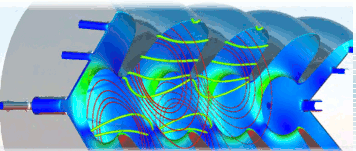
\includegraphics[height=.85cm]{figs/visit-logos/VisIt-02}} \hspace{-.85cm}{\bf \textcolor{lightgray}{VisIt}}: Import Data}

\begin{columns}
\begin{column}{6.25cm}
        \textcolor{DarkRed}{*} Importing datasets

        \textcolor{DarkBlue}{$\blacktriangleright$}
        \framebox{File} $\rightarrow$ \framebox{\bf Open file...}

        \hspace{2mm} $\mapsto$ choose data file {\small (eg. ``\textcolor{gray}{noise.silo}'')}

        \pause
        \vspace{2mm}
        \begin{beamerboxesrounded}[upper=block head,lower=block body,shadow=true]{\ding{231} Become available}
                \hspace{2mm}
                \ding{232} \textcolor{DarkBlue}{Active source}: ``\textcolor{gray}{noise.silo}''

                \hspace{2mm}
                \ding{232} \textcolor{DarkBlue}{Add button}
        \end{beamerboxesrounded}

        \pause
        \vspace{2mm}
        \textcolor{DarkBlue}{$\blacktriangleright$}
        \framebox{File} $\rightarrow$ \framebox{\bf File information...}
\end{column}
\begin{column}{5.5cm}
        \textcolor{DarkRed}{*} Restoring a previous session

        \vspace{2.5mm}
        \textcolor{DarkBlue}{$\blacktriangleright$}
        \framebox{File} $\rightarrow$ \framebox{\bf Restore session...}
        \\
        loads the previous state of the given session (\textbf{that needs to be specifically saved})

        \vspace{3.5mm}
        \textcolor{DarkBlue}{$\blacktriangleright$}
        \framebox{File} $\rightarrow$ \framebox{\bf Restore session w/sources...}
        \\
        extremely useful for re-identifiying datasets that could have been moved or renamed
        %\centering
        %\includegraphics[width=.85\columnwidth]{figs/}
\end{column}
\end{columns}
\pause
\vspace{2mm}
\begin{beamerboxesrounded}[upper=block head,lower=block body,shadow=true]{}
Be aware, that VisIt, by default won't save your work (session) nor ask you when you try to exit the program!
\end{beamerboxesrounded}
\end{frame}




\subsection{Contours: Iso-Surfaces \& Iso-Curves}
\begin{frame}
\frametitle{\href{https://wci.llnl.gov/simulation/computer-codes/visit/}{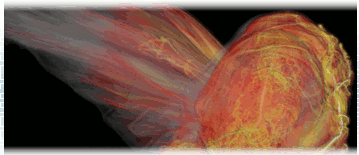
\includegraphics[height=.85cm]{figs/visit-logos/VisIt-03}} \hspace{-.85cm}{\bf \textcolor{lightgray}{VisIt}}: Contours}

\begin{columns}
\begin{column}{5cm}
        \textcolor{DarkBlue}{$\blacktriangleright$}
        \framebox{Add$_\blacktriangledown$} $\rightarrow$ \framebox{Contours}

        \hspace{5.5mm}
        $\leadsto$ \framebox{\textcolor{DarkGreen}{\it hardyglobal}}

        \hspace{5.5mm}
        $\rightarrow$ \framebox{\textcolor{DarkBlue}{Draw}}

        \centering
        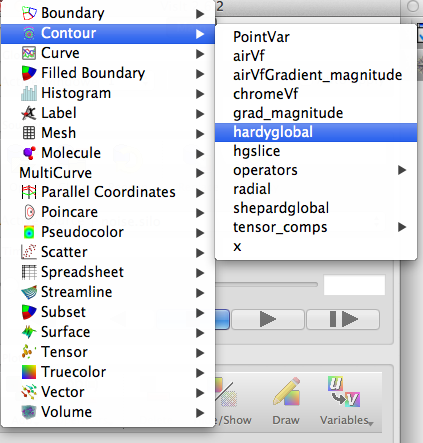
\includegraphics[width=\columnwidth]{figs/visit-pract/VisIt_contour}
\end{column}
\begin{column}{6.5cm}
        \centering
        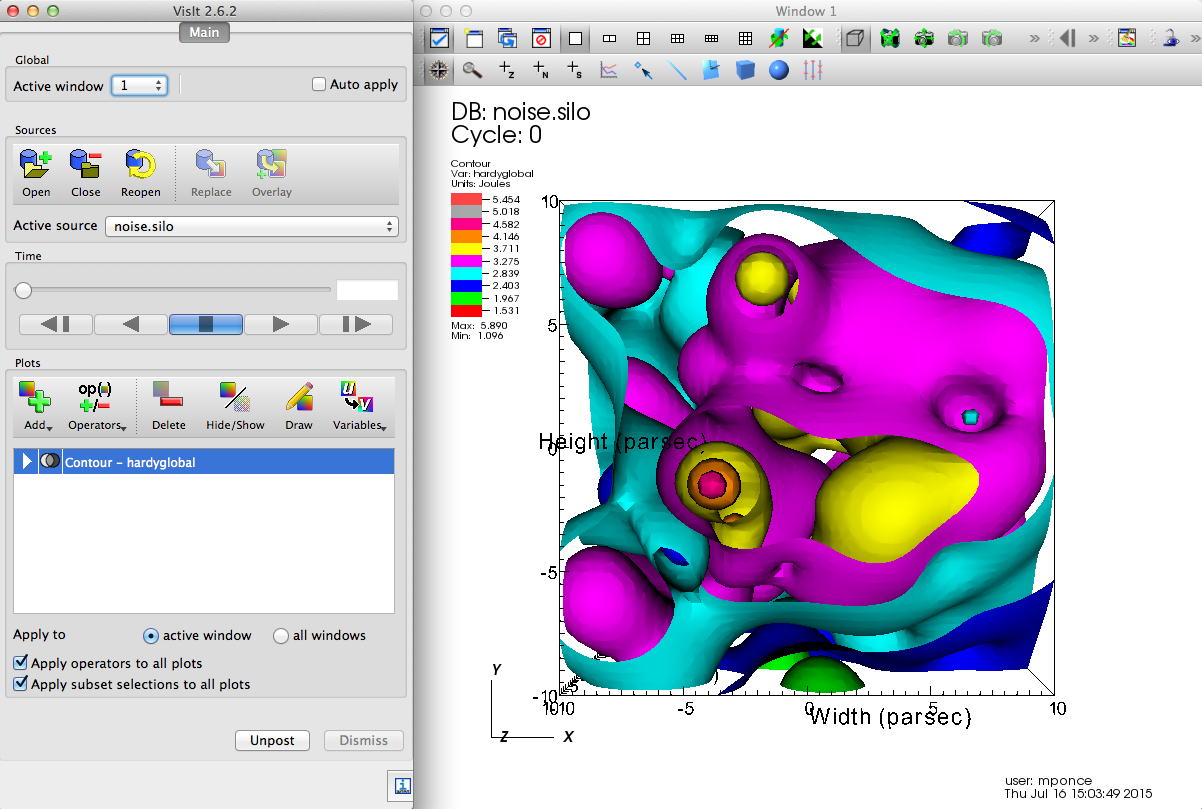
\includegraphics[width=\columnwidth]{figs/visit-pract/VisIt_contour1a}
\end{column}
\end{columns}
\end{frame}


\begin{frame}
\frametitle{\href{https://wci.llnl.gov/simulation/computer-codes/visit/}{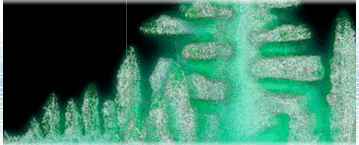
\includegraphics[height=.85cm]{figs/visit-logos/VisIt-04}} \hspace{-.85cm}{\bf \textcolor{lightgray}{VisIt}}: Contours}

\begin{columns}
\begin{column}{6cm}
        \textcolor{DarkBlue}{\ding{224}}
        double-click on \textcolor{DarkGreen}{Contour-hardyglobal}

        \pause
        \textcolor{DarkBlue}{\ding{224}}
        under \textcolor{DarkBlue}{Select by}, choose \framebox{\textcolor{DarkGreen}{N levels}} = \textcolor{blue}{5} \Enter

        \pause
        \textcolor{DarkBlue}{\ding{224}}
        Change \textcolor{DarkBlue}{opacity levels}, eg: 100\%, 60\%, 60\%, 48\%, 24\%

        \centering
        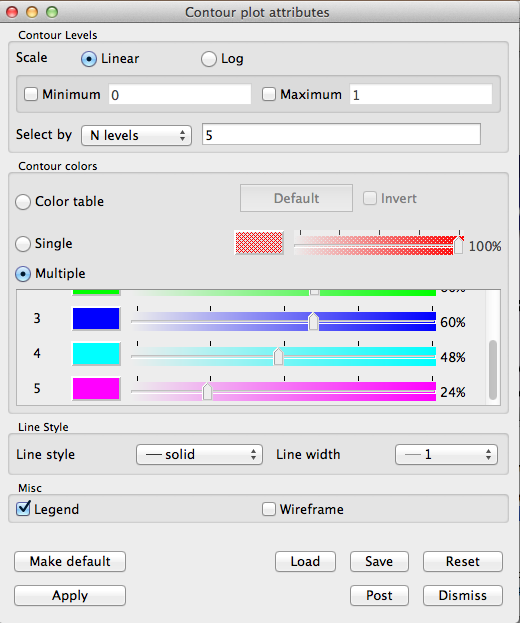
\includegraphics[width=.65\columnwidth]{figs/visit-pract/VisIt_contour-props}
\end{column}
\begin{column}{5.5cm}
        %\pause
        \textcolor{DarkBlue}{\ding{224}}
        \framebox{Apply}
        \&
        \framebox{Dismiss}

        \vspace{3mm}
        %\centering
        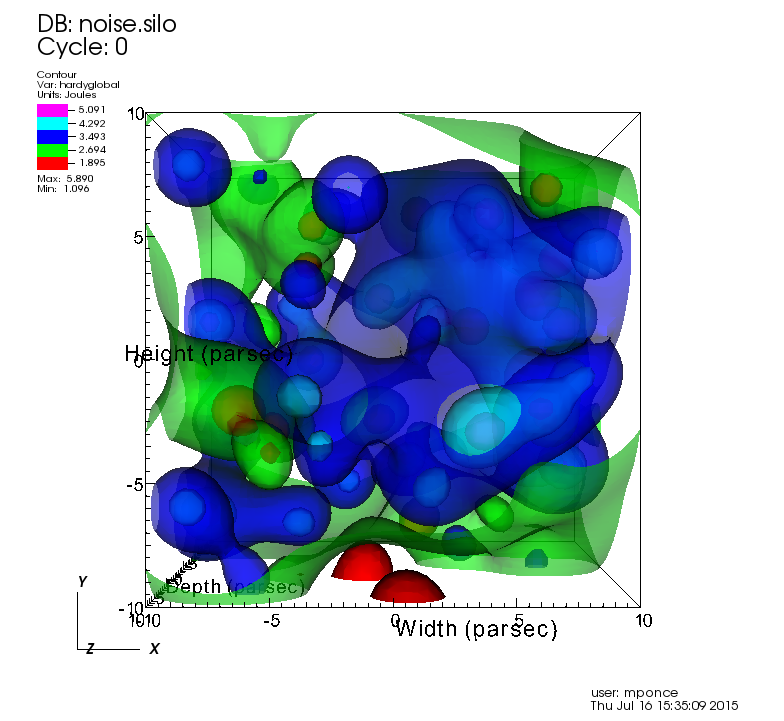
\includegraphics[width=\columnwidth]{figs/visit-pract/VisIt_contour1b}

        \pause
        \vspace{3mm}
        %\left
        \textcolor{DarkBlue}{\ding{224}}
        \framebox{Hide/Show}
        or
        \framebox{Delete}
\end{column}
\end{columns}
\end{frame}

\begin{frame}
\frametitle{\href{https://wci.llnl.gov/simulation/computer-codes/visit/}{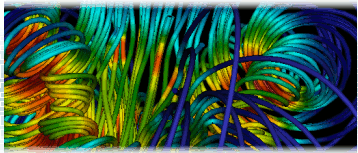
\includegraphics[height=.85cm]{figs/visit-logos/VisIt-01}} \hspace{-.85cm}{\bf \textcolor{lightgray}{VisIt}}: PseudoColor \& IsoSurfaces}
\vspace{-1.85mm}
\begin{columns}
\begin{column}{6cm}
        \textcolor{DarkBlue}{\ding{224}}
        \framebox{Add$_\blacktriangledown$} $\rightarrow$ \framebox{\textcolor{DarkRed}{\bf Pseudocolor}}

        \hspace{5.5mm}
        $\leadsto$ \framebox{\textcolor{DarkGreen}{\it hardyglobal}}

        \hspace{5.5mm}
        $\rightarrow$ \framebox{\textcolor{DarkBlue}{Draw}}

        \centering
        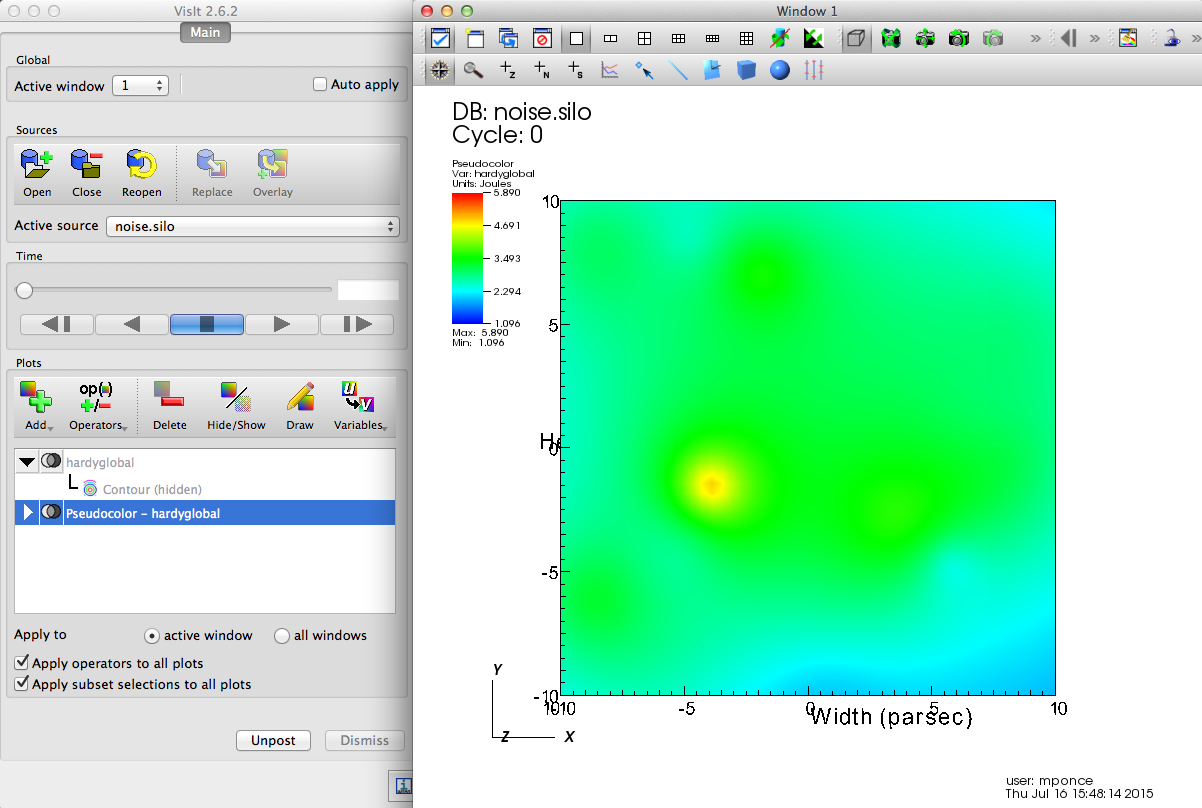
\includegraphics[width=\columnwidth]{figs/visit-pract/VisIt_pseudocolor}
\end{column}
\begin{column}{6cm}
        \pause
        \textcolor{DarkBlue}{\ding{224}}
        \framebox{Operators$_\blacktriangledown$}
                $\rightarrow$ \framebox{\bf Slicing}

        \hspace{5.5mm}
        $\rightarrow$ \framebox{\textcolor{DarkRed}{\bf Isosurface}}

        \hspace{5.5mm}
        $\rightarrow$ \framebox{\textcolor{DarkBlue}{Draw}}

        \centering
        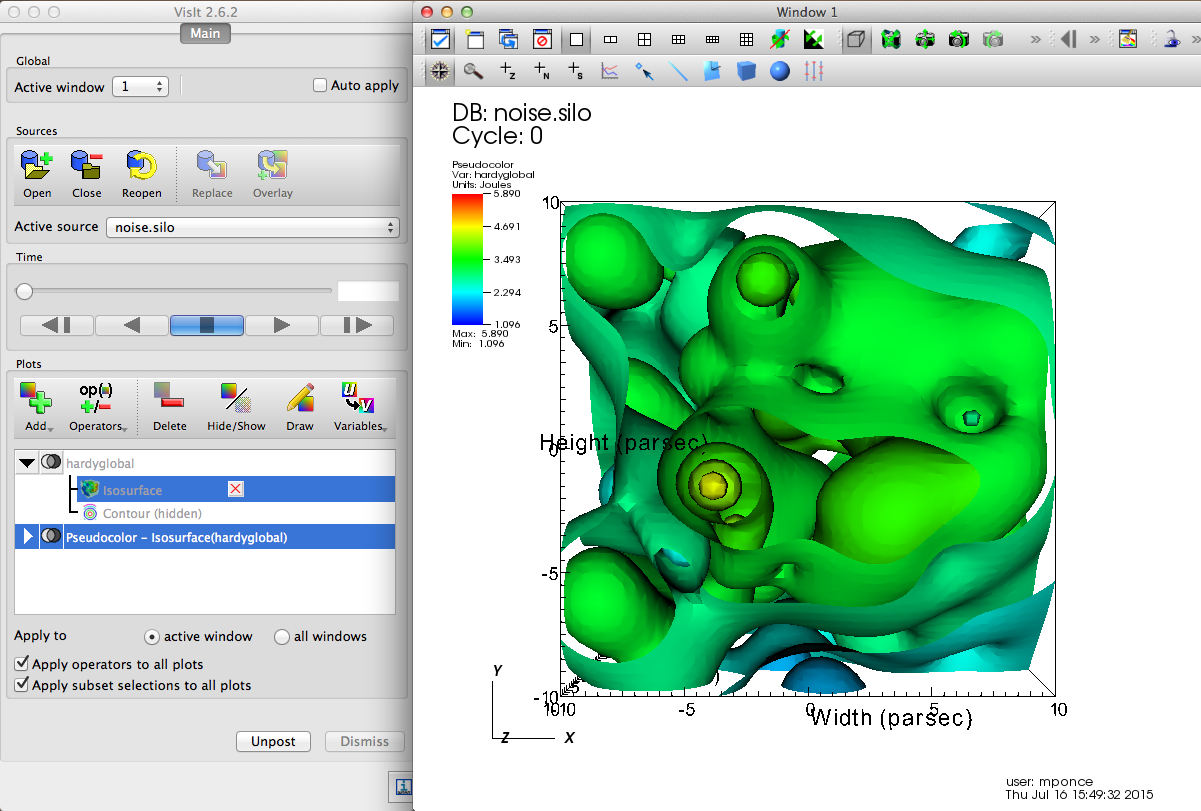
\includegraphics[width=\columnwidth]{figs/visit-pract/VisIt_pseudocolor-isosurf}
\end{column}
\end{columns}

\pause
\vspace{2mm}
\textcolor{DarkBlue}{\ding{224}}
        click $\blacktriangleright$ to expand, double click on [\textcolor{DarkBlue}{Isosurface}]

\hspace{4mm}
\textcolor{DarkBlue}{\ding{223}}
under \textcolor{DarkBlue}{Select by}, choose \framebox{\textcolor{DarkGreen}{Percent (s)}} = \textcolor{blue}{50} \Enter \& \framebox{Dismiss}


\pause
\vspace{2mm}
\textcolor{DarkBlue}{\ding{224}}
        change the \textcolor{DarkRed}{opacity} of [\textcolor{DarkBlue}{Pseudocolor}]
\end{frame}


\begin{frame}
\frametitle{\href{https://wci.llnl.gov/simulation/computer-codes/visit/}{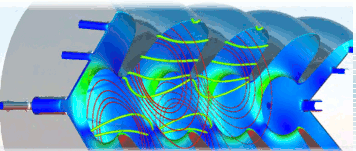
\includegraphics[height=.85cm]{figs/visit-logos/VisIt-02}} \hspace{-.85cm}{\bf \textcolor{lightgray}{VisIt}}: PseudoColor \& IsoSurfaces}
\vspace{-1.5mm}
\begin{columns}%[T]
\begin{column}{9cm}
        \centering
        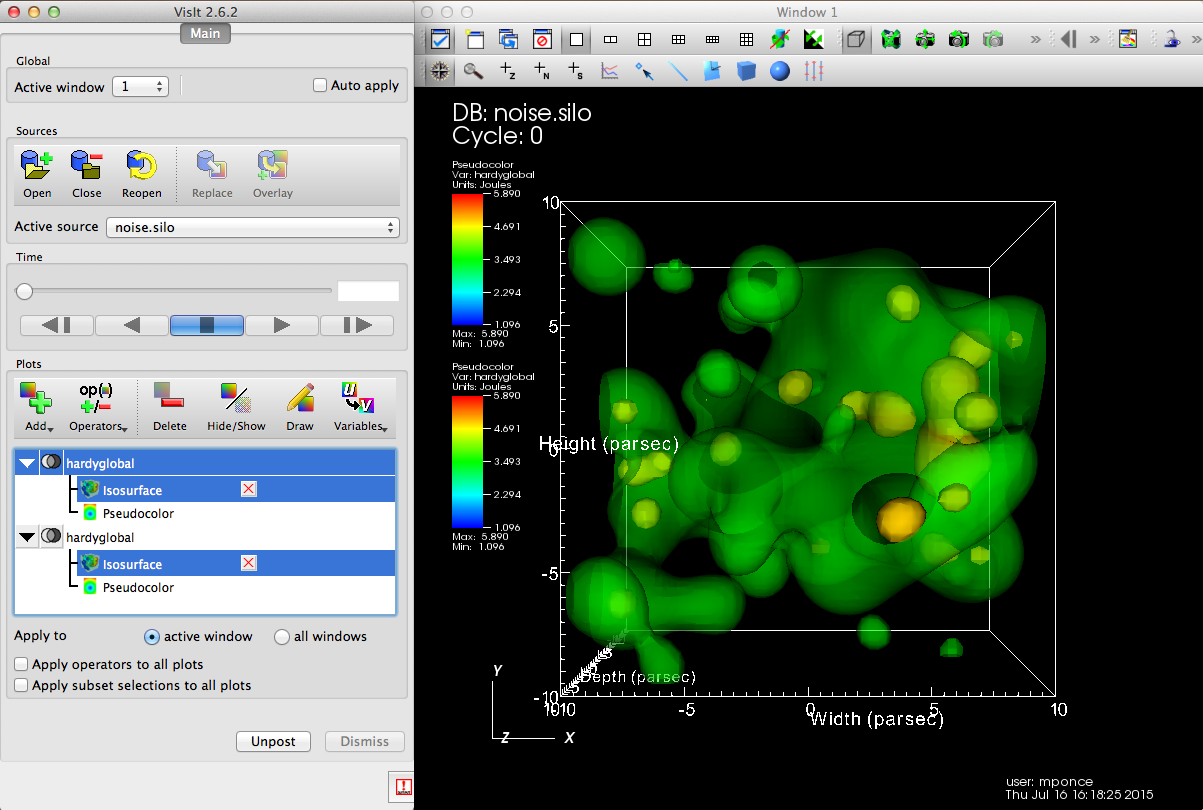
\includegraphics[width=\columnwidth]{figs/visit-pract/VisIt_pseudocolor-isosurf_2}
\end{column}
\begin{column}{3cm}
        \pause
        \textcolor{DarkBlue}{\ding{224}}
        unselect the [\textcolor{DarkBlue}{Apply ...}] check-boxes

        \vspace{2mm}
        \textcolor{DarkBlue}{\ding{224}} add 1 more
                \textcolor{DarkRed}{Pseudocolor}
                +\textcolor{DarkRed}{\bf Isosurface},
        \\
        %\hspace{1.5mm}
        w/\textcolor{DarkBlue}{Percent(s)=80}
        \& adjust its
        \textcolor{DarkBlue}{opacity}
\end{column}
\end{columns}

\pause
\vspace{2mm}
\textcolor{DarkBlue}{\ding{224}}
        \textcolor{blue}{clipping} \ding{223} select/check the [\textcolor{DarkBlue}{Apply...}] boxes

%\vspace{1mm}
\textcolor{DarkBlue}{\ding{224}}
        \framebox{Operators$_\blacktriangledown$}
                $\rightarrow$ \framebox{\bf Selection}
        %\hspace{5.5mm}
        $\rightarrow$ \framebox{\textcolor{DarkRed}{\bf Clip}}

        \hspace{5mm}
        \ding{223} choose \textcolor{DarkBlue}{combinations of $\ne$ planes} to modify the $\ll$clip$\gg$
\end{frame}






%\handsonEnv
\begin{frame}
\frametitle{\href{https://wci.llnl.gov/simulation/computer-codes/visit/}{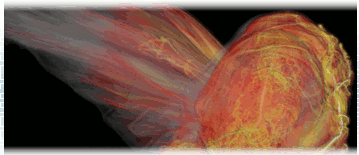
\includegraphics[height=.85cm]{figs/visit-logos/VisIt-03}} \hspace{-.85cm}{\bf \textcolor{lightgray}{VisIt}}: General Remarks}

\begin{beamerboxesrounded}[upper=block head,lower=block body,shadow=true]{}
        \textcolor{DarkBlue}{\ding{231}} operators/plots can be removed
                \framebox{\textcolor{DarkBlue}{\bf Delete}}
                --or--
                hidden \framebox{\textcolor{DarkBlue}{\bf Hide/Show}}

        \textcolor{DarkBlue}{\ding{231}} save your work {\bf frequently}:
                \framebox{File} $\rightarrow$ \framebox{\textcolor{DarkBlue}{\bf Save session...}}
\end{beamerboxesrounded}

%\begin{comment}
%\pause
%\vspace{3mm}
%\begin{beamerboxesrounded}[upper=block head,lower=block body,shadow=true]{\bf Hands-on...}%Assignment ii}
%%        \textcolor{DarkRed}{\ding{231}} try loading some of the datasets we used with ParaView [{\small \textcolor{gray}{\tt headsq.vtk}, \textcolor{gray}{\tt testRectilinearGrid.vtk}, \textcolor{gray}{\tt disk\_out\_ref.ex2}, ...}] --or-- your own data!!!
%	\textcolor{DarkRed}{\ding{231}} Load some of the other datasets, eg.
%		[{\small \textcolor{gray}{\tt headsq.vtk}, \textcolor{gray}{\tt testRectilinearGrid.vtk}, \textcolor{gray}{\tt disk\_out\_ref.ex2}, ...}]
%		--or-- your own data!!!
%
%	\textcolor{DarkRed}{\ding{231}} Try to explore the data and visualize it, using some of the tools we have discussed
%
%	\textcolor{DarkRed}{\ding{231}} If you have used other visualization packages, compare how easy and
%		whether it is possible or not, to obtain similar results, let's say, to ParaView or VAPOR for instance...
%
%	\textcolor{DarkRed}{\ding{231}} also which one, results more intuitive, elegant, useful for you and your research
%\end{beamerboxesrounded}
%\end{comment}
\end{frame}
%\resetEnv
%\basicEnv






\subsection{Slices}
\begin{frame}
\frametitle{\href{https://wci.llnl.gov/simulation/computer-codes/visit/}{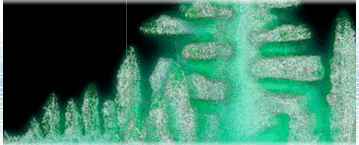
\includegraphics[height=.85cm]{figs/visit-logos/VisIt-04}} \hspace{-.85cm}{\bf \textcolor{lightgray}{VisIt}}: Slices}
\begin{columns}
\begin{column}{8cm}
\begin{beamerboxesrounded}[upper=block head,lower=block body,shadow=true]{Slicing Isosurfaces}
	\textcolor{DarkBlue}{\ding{224}} 
		\framebox{Operators$_\blacktriangledown$}
			$\rightarrow$ \framebox{\bf Slicing}
			$\rightarrow$ \framebox{\bf \textcolor{DarkBlue}{Slice}}

	\textcolor{DarkBlue}{\ding{224}}
		double-click on [\textcolor{DarkBlue}{Slice}]

	\hspace{3.5mm}
	\ding{223}
		try choosing different \textcolor{DarkRed}{axes} 

		\hspace{7.75mm}
		\& \textcolor{DarkRed}{Project to 2D}

	\hspace{3.5mm}
	\ding{223}
		try also the other types of slices
\end{beamerboxesrounded}
\end{column}
\begin{column}{3.5cm}
	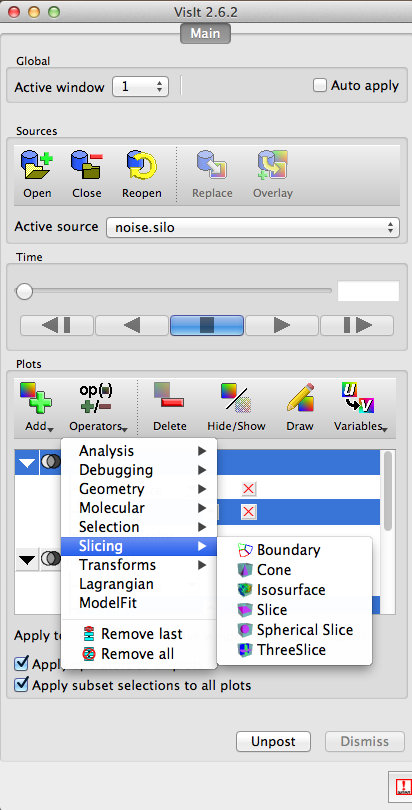
\includegraphics[width=\columnwidth]{figs/visit-pract/VisIt_sliceIsosurf}
\end{column}
\end{columns}
\end{frame}


\subsection{Vector Fields: Glyphs \& Streamlines}
\begin{frame}
\frametitle{\href{https://wci.llnl.gov/simulation/computer-codes/visit/}{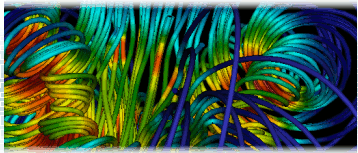
\includegraphics[height=.85cm]{figs/visit-logos/VisIt-01}} \hspace{-.85cm}{\bf \textcolor{lightgray}{VisIt}}: Vector Field representations -- {Glyphs}}
\begin{columns}
\begin{column}{9cm}
\begin{beamerboxesrounded}[upper=block head,lower=block body,shadow=true]{\textcolor{DarkRed}{\ding{232}} \textcolor{blue}{Glyphs}}
	\textcolor{DarkBlue}{\ding{224}} 
		\framebox{Add$_\blacktriangledown$}
			$\rightarrow$ \framebox{\bf \textcolor{DarkBlue}{Vector}}
			$\leadsto$ \framebox{\textcolor{DarkGreen}{\it airVfGradient}}

	\hspace{3.5mm}
	\ding{223}
		\framebox{Apply} \& \framebox{Dismiss}

	\vspace{2mm}
	\textcolor{DarkBlue}{\ding{224}} 
		double-click on [\textcolor{DarkBlue}{Vector}]

	\vspace{1.25mm}
	\hspace{3.5mm}
	\ding{223}
		set \textcolor{DarkBlue}{Vector amount} $\leadsto$ \textcolor{DarkOrange}{1000}

	\vspace{1.25mm}
	\hspace{3.5mm}
	\ding{223}
		more \textit{properties} in [\textcolor{DarkBlue}{Form}] \& [\textcolor{DarkBlue}{Rendering}]
\end{beamerboxesrounded}
\end{column}
\begin{column}{2.75cm}
\end{column}
\end{columns}
\end{frame}


\begin{frame}
\frametitle{\href{https://wci.llnl.gov/simulation/computer-codes/visit/}{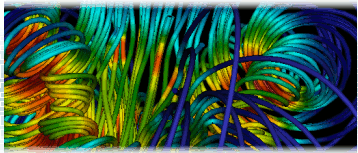
\includegraphics[height=.85cm]{figs/visit-logos/VisIt-01}} \hspace{-.85cm}{\bf \textcolor{lightgray}{VisIt}}: Vector Field representations -- {Streamlines}}
\begin{columns}
\begin{column}{9cm}
\begin{beamerboxesrounded}[upper=block head,lower=block body,shadow=true]{\textcolor{DarkRed}{\ding{232}} \textcolor{blue}{Streamlines}}
	\textcolor{DarkBlue}{\ding{224}} 
		\framebox{Add$_\blacktriangledown$}
			$\rightarrow$ \framebox{\bf \textcolor{DarkBlue}{Streamline}}
			$\leadsto$ \framebox{\textcolor{DarkGreen}{grad}}

	\vspace{2mm}
	\textcolor{DarkBlue}{\ding{224}} 
		double-click on [\textcolor{DarkBlue}{Streamline}]

	\vspace{.75mm}
	\hspace{3.5mm}
	\ding{223}
		set \textcolor{DarkBlue}{Source type} $\leadsto$ \textcolor{DarkOrange}{plane}

	\hspace{3.5mm}
	\ding{223}
		increase \textcolor{DarkBlue}{samples}/\textcolor{DarkBlue}{distance} along axes$\leadsto$\textcolor{DarkOrange}{15/20}

	\hspace{3.5mm}
	\ding{223}
		\textcolor{DarkBlue}{Streamline direction} $\leadsto$ \textcolor{DarkOrange}{both}
	\end{beamerboxesrounded}
\end{column}
\begin{column}{3.5cm}
	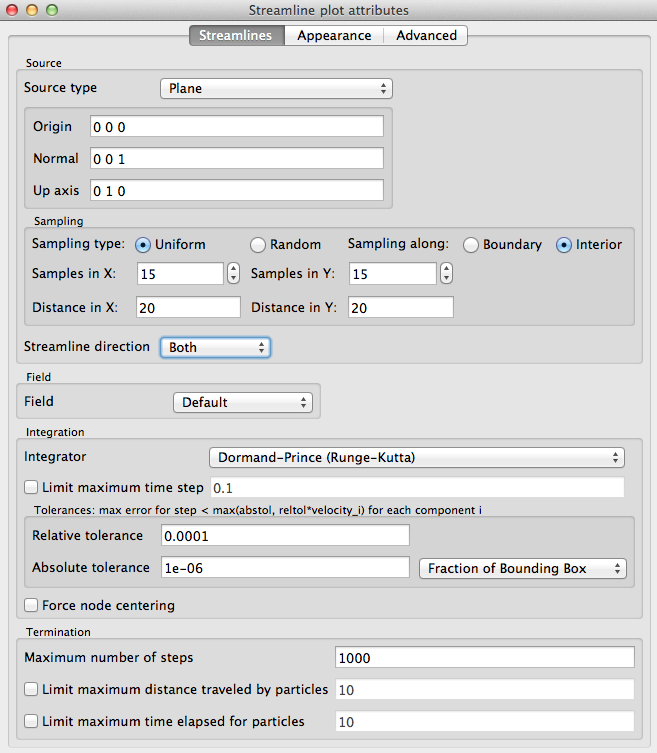
\includegraphics[width=\columnwidth]{figs/visit-pract/VisIt_streamlines-attribs}
\end{column}
\end{columns}
\begin{columns}
\begin{column}{11cm}
	\pause
	\begin{beamerboxesrounded}[upper=block head,lower=block body,shadow=true]{}
	\vspace{1.75mm}
	\hspace{3.5mm}
	\ding{223}
		in [\textcolor{DarkBlue}{Appearance}],  \textcolor{DarkBlue}{Drawn as} $\leadsto$ \textcolor{DarkOrange}{Tubes}, w/\textcolor{DarkOrange}{Radius $\leadsto$ 0.005}
	%\end{beamerboxesrounded}

	\pause
	%\begin{beamerboxesrounded}[upper=block head,lower=block body,shadow=true]{}
	\hspace{3.5mm}
	\ding{223}
		[\textcolor{DarkBlue}{Data Value}] $\leadsto$ \textcolor{DarkOrange}{Variable} $\rightarrow$ \textcolor{DarkGreen}{\it hardyglobal}
	%\end{beamerboxesrounded}

	\pause
	%\begin{beamerboxesrounded}[upper=block head,lower=block body,shadow=true]{}
	\hspace{3.5mm}
	\ding{223}
		[\textcolor{DarkBlue}{Color Table}] $\leadsto$ \textcolor{DarkOrange}{bluehot}
	\ding{223} \framebox{Apply}
	\end{beamerboxesrounded}

	\pause
	\begin{beamerboxesrounded}[upper=block head,lower=block body,shadow=true]{}
	\hspace{3.5mm}
	\ding{223}
		experiment with \textcolor{DarkBlue}{Shown seeds}
\end{beamerboxesrounded}
\end{column}
\begin{column}{2cm}
\end{column}
\end{columns}
\end{frame}


\begin{frame}
\frametitle{\href{https://wci.llnl.gov/simulation/computer-codes/visit/}{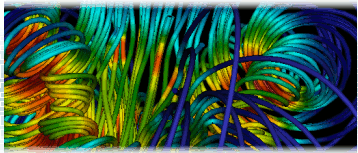
\includegraphics[height=.85cm]{figs/visit-logos/VisIt-01}} \hspace{-.85cm}{\bf \textcolor{lightgray}{VisIt}}: Vector Field representations -- {Streamlines}}
	\centering
	%	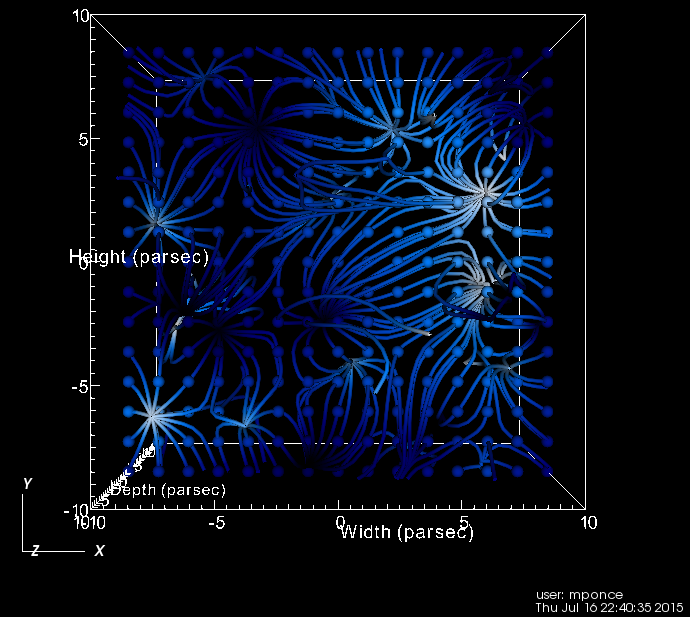
\includegraphics[width=0.3\columnwidth]{figs/VisIt_streamlines-01a}
	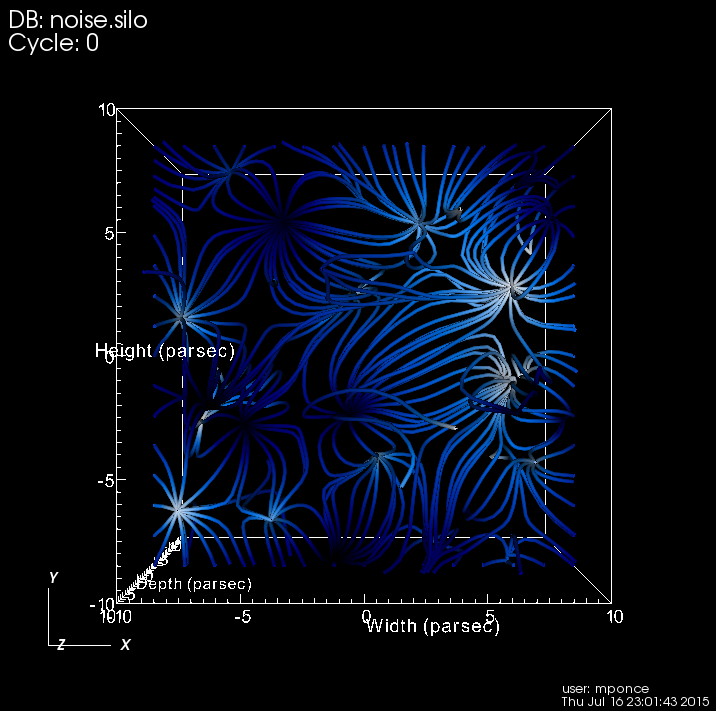
\includegraphics[width=0.45\columnwidth]{figs/visit-pract/VisIt_streamlines-01b}
	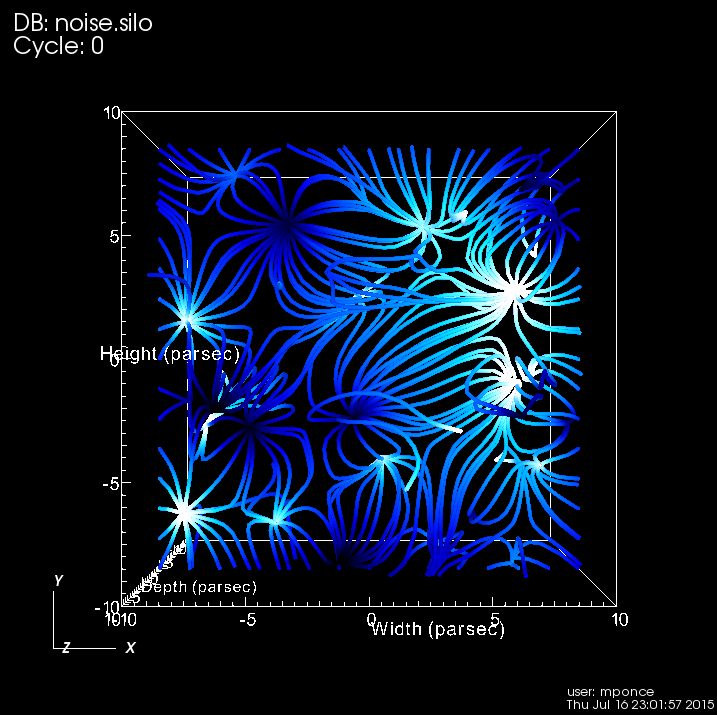
\includegraphics[width=0.45\columnwidth]{figs/visit-pract/VisIt_streamlines-01c}

\end{frame}



\begin{frame}
\frametitle{\href{https://wci.llnl.gov/simulation/computer-codes/visit/}{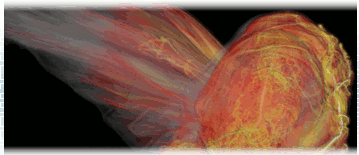
\includegraphics[height=.85cm]{figs/visit-logos/VisIt-03}} \hspace{-.85cm}{\bf \textcolor{lightgray}{VisIt}}: Slices}
\begin{columns}
\begin{column}{6.5cm}
\begin{beamerboxesrounded}[upper=block head,lower=block body,shadow=true]{}
	\textcolor{DarkBlue}{\ding{224}} 
		\framebox{Add$_\blacktriangledown$}
			$\rightarrow$ \framebox{\bf \textcolor{DarkBlue}{Pseudocolor}}

			\hspace{5mm}
			$\leadsto$ \framebox{\textcolor{DarkGreen}{grad\_magnitude}}

	\pause
	\textcolor{DarkBlue}{\ding{224}} 
		\framebox{Operator$_\blacktriangledown$}
			$\rightarrow$ \framebox{\bf Slice}
			$\leadsto$ \framebox{\textcolor{DarkBlue}{\bf Slicing}}

	\pause
	\vspace{2mm}
	\textcolor{DarkBlue}{\ding{224}} 
		double-click on [\textcolor{DarkBlue}{Slice}]

	\vspace{.75mm}
	\hspace{3.5mm}
	\ding{223}
		select $\leadsto$ \textcolor{DarkOrange}{Z-axis}

	\hspace{3.5mm}
	\ding{223}
		unselct \textcolor{DarkBlue}{Project to 2D}

	\hspace{3.5mm}
	\ding{223}
		\framebox{Apply}

	\hspace{3.5mm}
	\ding{223}
		\framebox{Draw}

	\hspace{3.5mm}
	\ding{223}
		\framebox{Hide/Show}
	\end{beamerboxesrounded}
\end{column}
\begin{column}{5.5cm}
	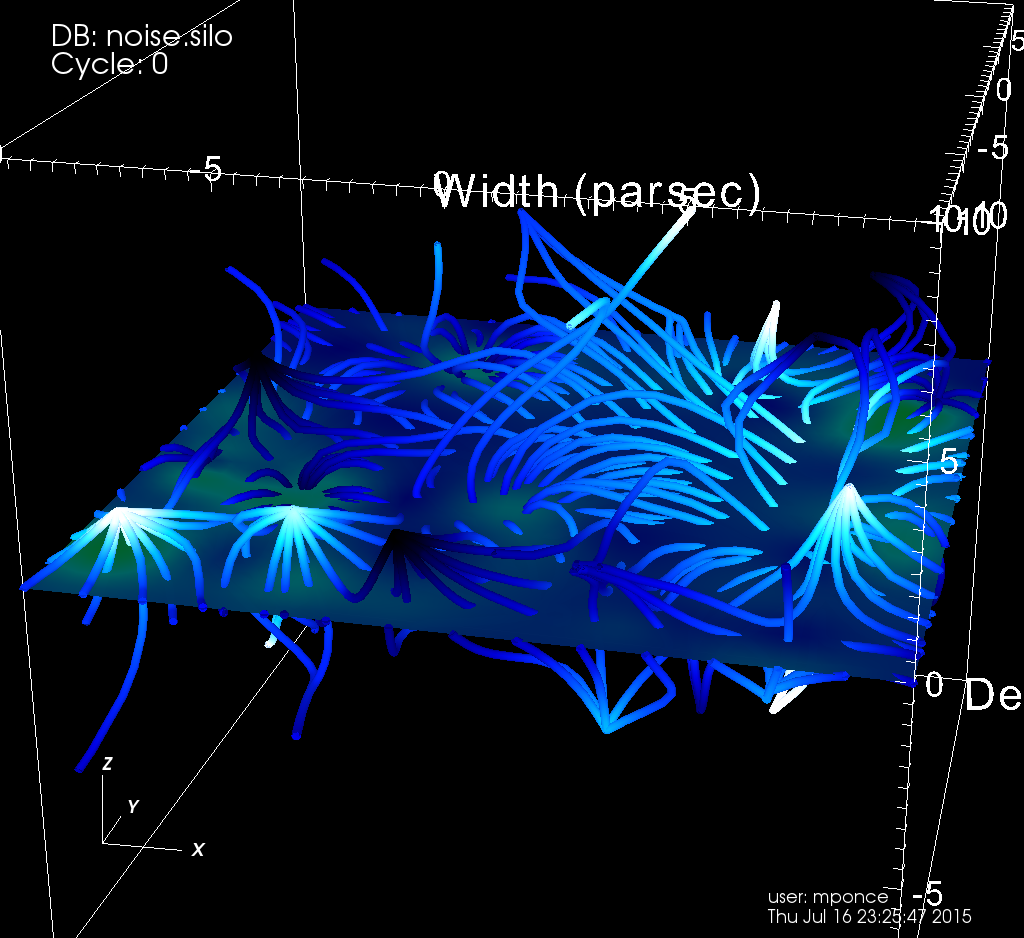
\includegraphics[width=\columnwidth]{figs/visit-pract/VisIt_slice01a}
\end{column}
\end{columns}
\end{frame}


\subsection{Volume Rendering}
\begin{frame}
\frametitle{\href{https://wci.llnl.gov/simulation/computer-codes/visit/}{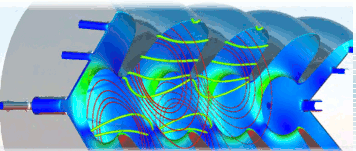
\includegraphics[height=.85cm]{figs/visit-logos/VisIt-02}} \hspace{-.85cm}{\bf \textcolor{lightgray}{VisIt}}: Volume Rendering}
\begin{columns}
\begin{column}{6.25cm}
\begin{beamerboxesrounded}[upper=block head,lower=block body,shadow=true]{}
	\textcolor{DarkBlue}{\ding{224}} 
		\framebox{Add$_\blacktriangledown$}
			$\rightarrow$ \framebox{\bf \textcolor{DarkBlue}{Volume}}

			\hspace{5mm}
			$\leadsto$ \framebox{\textcolor{DarkGreen}{grad\_magnitude}}

	\pause
	\vspace{2mm}
	\textcolor{DarkBlue}{\ding{224}} 
		double-click on [\textcolor{DarkBlue}{Volume}]

	\vspace{.75mm}
	\hspace{3.5mm}
	\ding{223}
		click on \textcolor{DarkOrange}{1D  Transfer Function}

	\hspace{3.5mm}
	\ding{223}
		change \textcolor{DarkBlue}{Transfer Fn}/\textcolor{DarkRed}{\bf Opacity}
	\end{beamerboxesrounded}

	\centering
	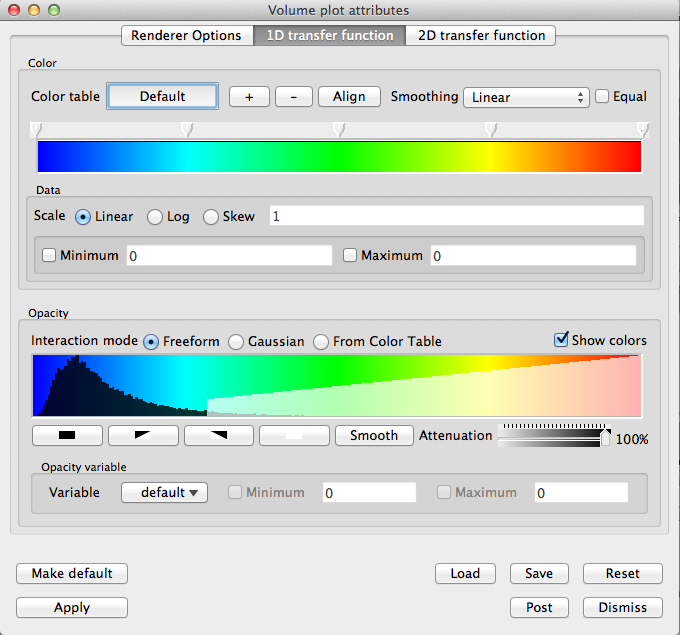
\includegraphics[width=.65\columnwidth]{figs/visit-pract/VisIt_1dTransfFn}
\end{column}
\begin{column}{5.5cm}
\begin{beamerboxesrounded}[upper=block head,lower=block body,shadow=true]{}
	\hspace{3.5mm}
	\ding{223}
		\framebox{Apply}

	\hspace{3.5mm}
	\ding{223}
		\framebox{Draw}
\end{beamerboxesrounded}

	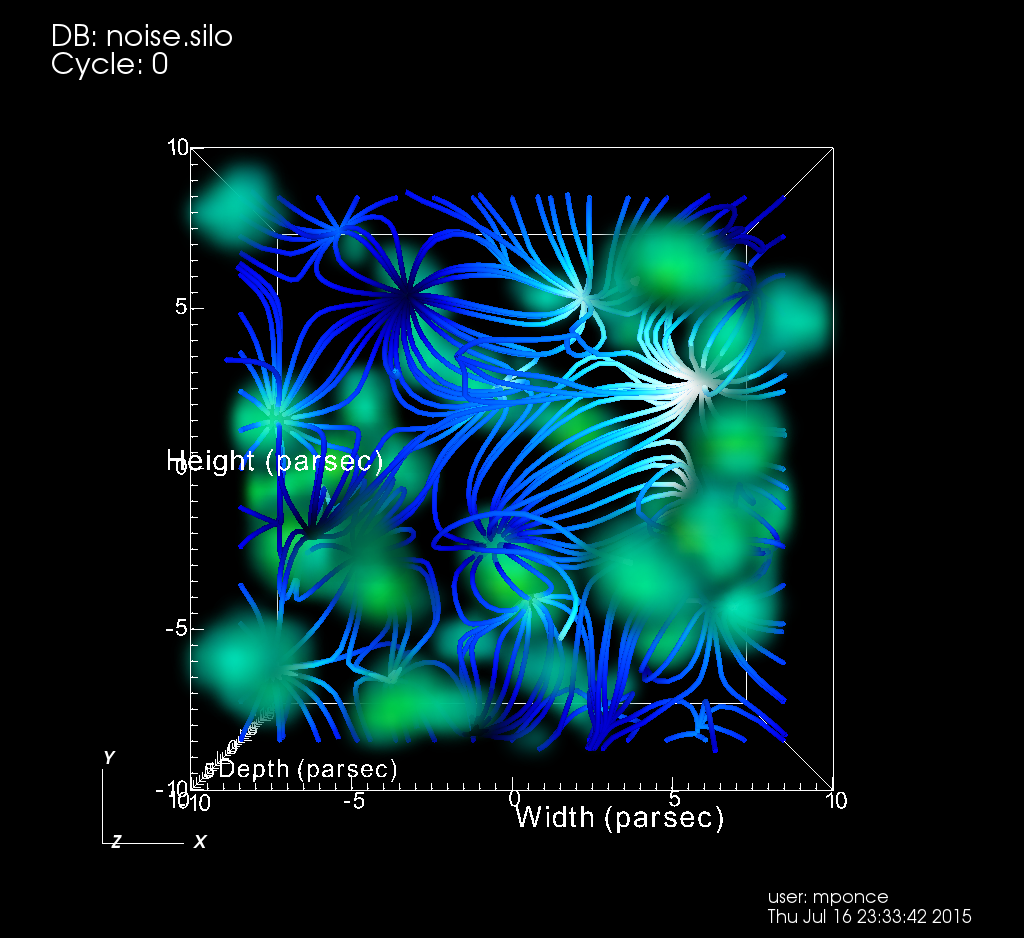
\includegraphics[width=\columnwidth]{figs/visit-pract/VisIt_volRendering01a}
\end{column}
\end{columns}
\end{frame}



\begin{frame}
\frametitle{\href{https://wci.llnl.gov/simulation/computer-codes/visit/}{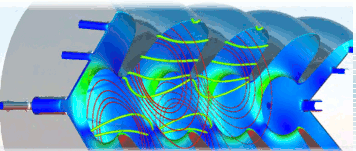
\includegraphics[height=.85cm]{figs/visit-logos/VisIt-02}} \hspace{-.85cm}{\bf \textcolor{lightgray}{VisIt}}: \textit{Aesthetics} \& Final Products}
\begin{columns}
\begin{column}{5.75cm}
	\begin{beamerboxesrounded}[upper=block head,lower=block body,shadow=true]{\textcolor{DarkRed}{\ding{232}} Legends, axes, ...}
		\textcolor{DarkBlue}{\ding{224}} 
		\framebox{Controls}
			$\rightarrow$ \framebox{\bf \textcolor{DarkBlue}{Annotantion...}}
	\end{beamerboxesrounded}
\end{column}
\begin{column}{5.5cm}
	\begin{beamerboxesrounded}[upper=block head,lower=block body,shadow=true]{\textcolor{DarkRed}{\ding{232}} ``hard-copies'': images, ...}
		\textcolor{DarkBlue}{\ding{224}} 
		\framebox{File}
			$\rightarrow$ \framebox{\bf \textcolor{DarkBlue}{Save Window}}
	\end{beamerboxesrounded}

\end{column}
\end{columns}

\vspace{5mm}
\begin{columns}
\begin{column}{12cm}
	\centering
	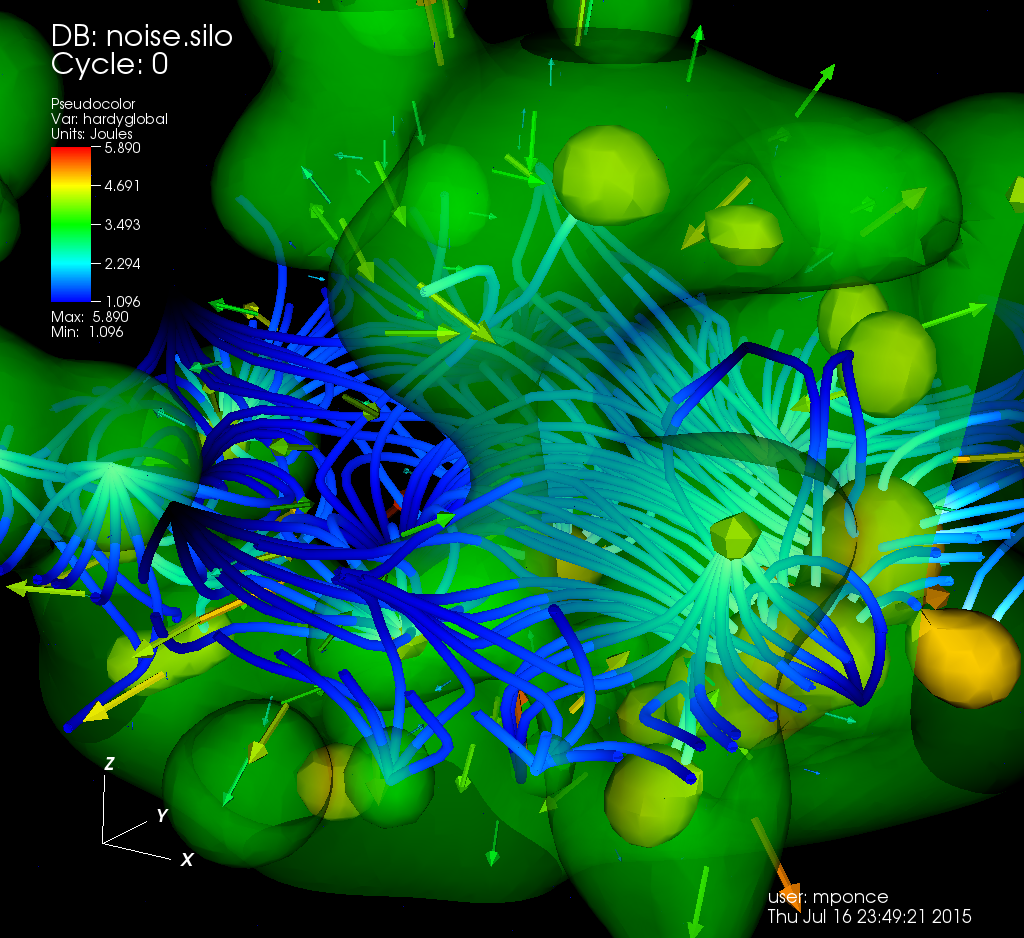
\includegraphics[width=.33\columnwidth]{figs/visit-pract/VisIt_mix01}
	~
	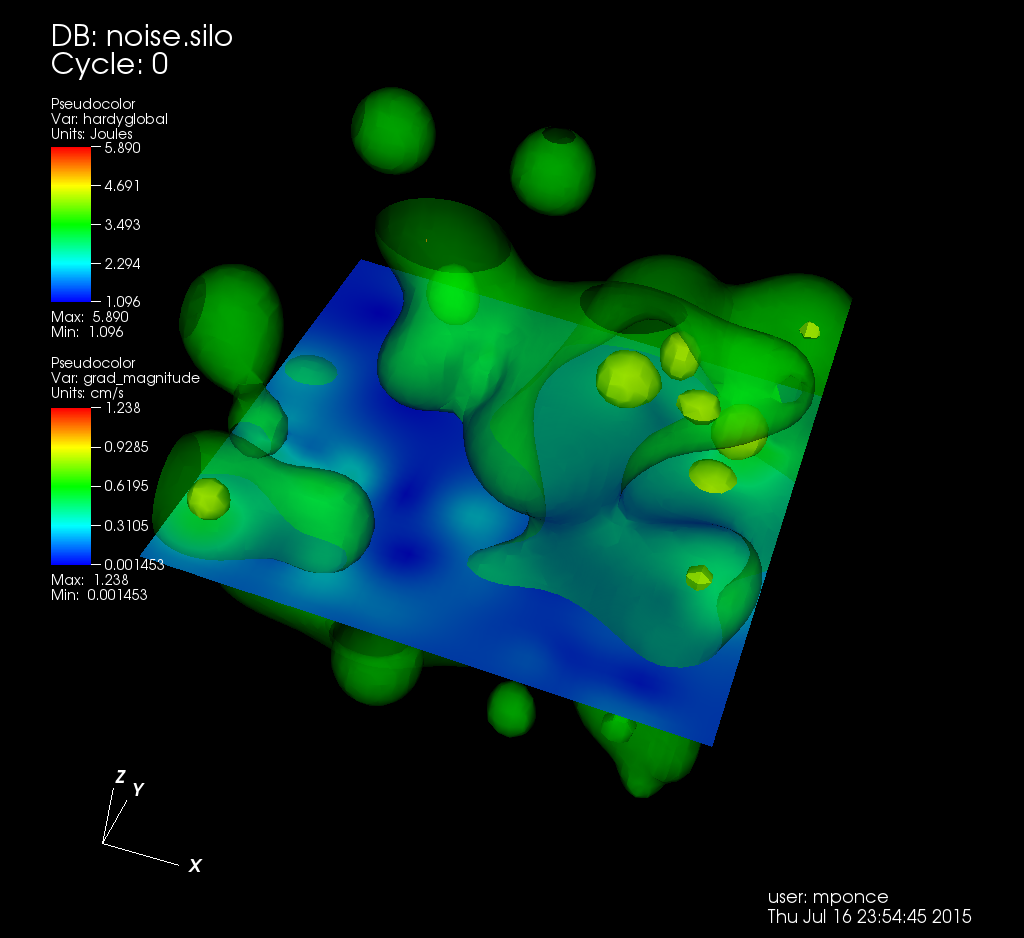
\includegraphics[width=.33\columnwidth]{figs/visit-pract/VisIt_mix02}
	~
	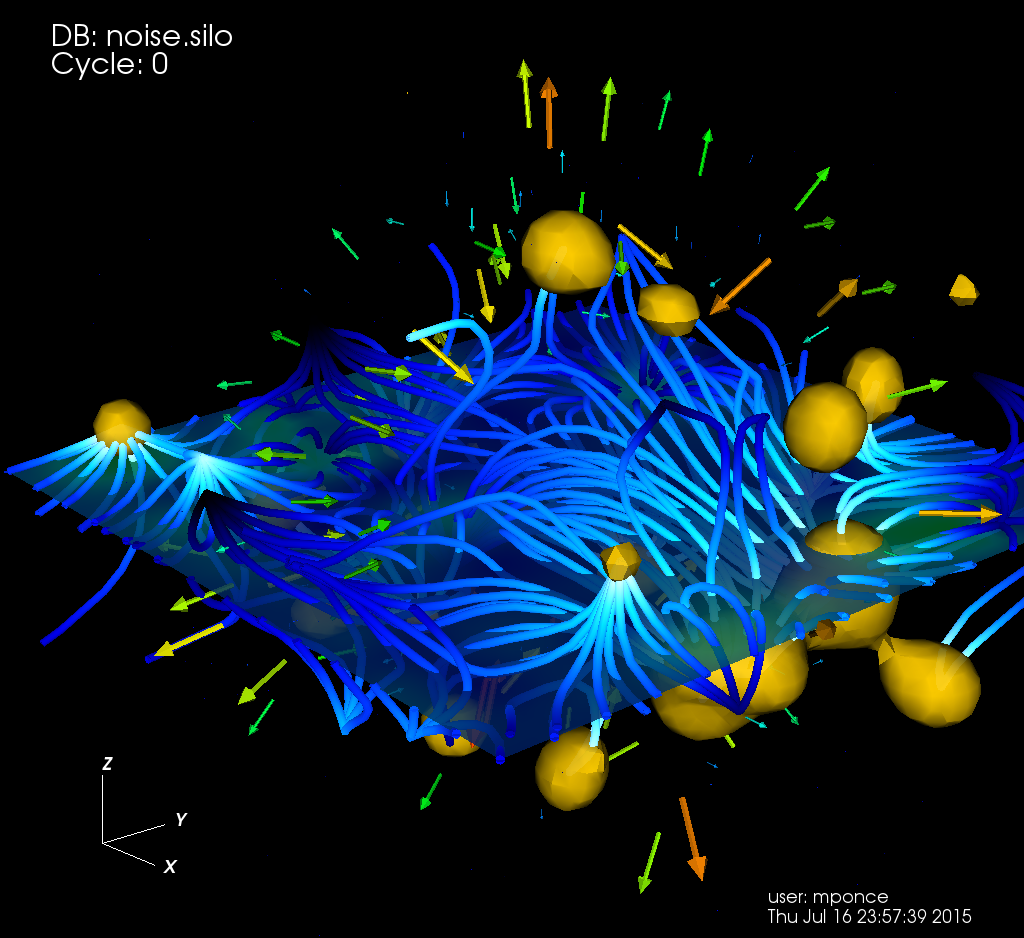
\includegraphics[width=.33\columnwidth]{figs/visit-pract/VisIt_mix03}
\end{column}
\end{columns}
\end{frame}



\subsection{Controls}
\begin{frame}
\frametitle{\href{https://wci.llnl.gov/simulation/computer-codes/visit/}{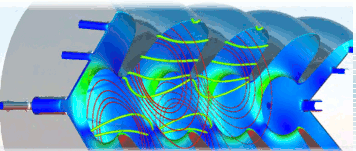
\includegraphics[height=.85cm]{figs/visit-logos/VisIt-02}} \hspace{-.85cm}{\bf \textcolor{DarkOrange}{VisIt}}: Controls}

\begin{columns}
\begin{column}{6.5cm}
	\textcolor{DarkBlue}{$\blacktriangleright$}
	\framebox{Controls} $\rightarrow$ \framebox{\bf Database Correlations...}

	\hspace{5mm} $\mapsto$ allow to create \textit{correlations} between $\neq$ datasets

	\pause
	\vspace{3.5mm}
	\textcolor{DarkBlue}{$\blacktriangleright$}
	\framebox{Controls} $\rightarrow$ \framebox{\bf Expressions...}

	\hspace{5mm} $\mapsto$ allow to create \textit{expresions} (new quantities) from variables/datasets

	\pause
	\vspace{3.5mm}
	\begin{beamerboxesrounded}[upper=block head,lower=block body,shadow=true]{\ding{231} Other interesting ones...}
		\hspace{2mm}
		\ding{232} \textcolor{DarkBlue}{Annotation...}

				\hspace{2mm}
		\ding{232} \textcolor{DarkBlue}{Lighting...}

		\hspace{2mm}
		\ding{232} \textcolor{DarkBlue}{View...}
	\end{beamerboxesrounded}
\end{column}
\begin{column}{5.25cm}
	\centering
	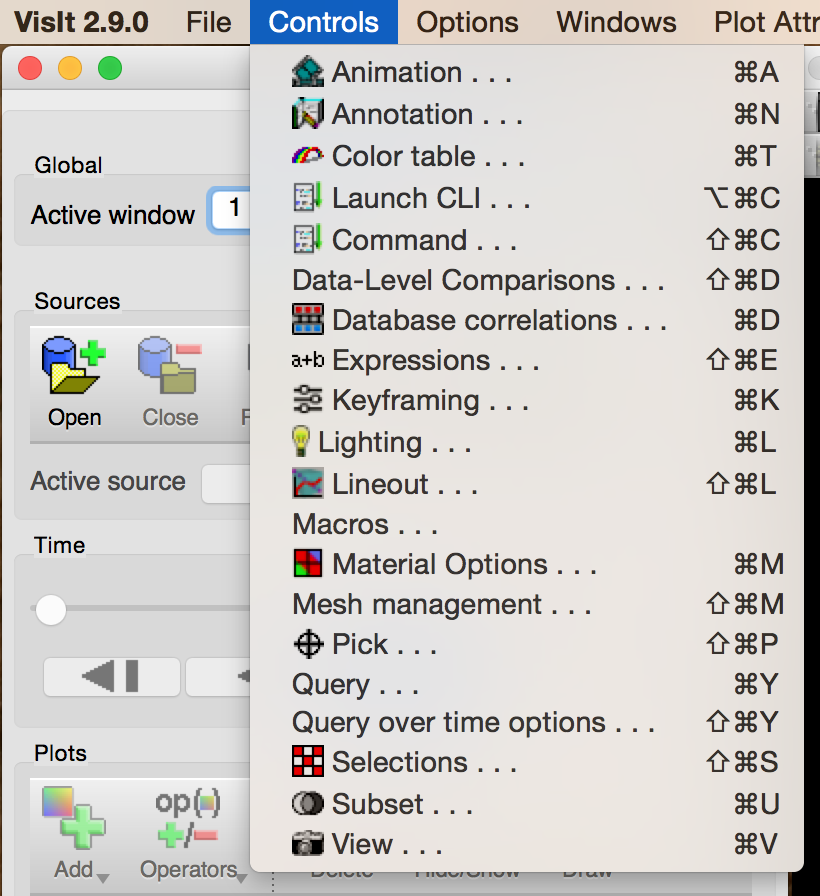
\includegraphics[width=.85\columnwidth]{figs/visit-guis/visit_ctrls}
\end{column}
\end{columns}
\end{frame}




